\documentclass[a4paper,14pt,oneside,openany]{memoir}

%%% Задаем поля, отступы и межстрочный интервал %%%

\usepackage[left=30mm, right=15mm, top=20mm, bottom=20mm]{geometry} % Пакет geometry с аргументами для определения полей
\pagestyle{plain} % Убираем стандарные для данного класса верхние колонтитулы с заголовком текущей главы, оставляем только номер страницы снизу по центру
\parindent=1.25cm % Абзацный отступ 1.25 см, приблизительно равно пяти знакам, как по ГОСТ
\usepackage{indentfirst} % Добавляем отступ к первому абзацу
%\linespread{1.3} % Межстрочный интервал (наиболее близко к вордовскому полуторному) - тут вместо этого используется команда OnehalfSpacing*

%%% Задаем языковые параметры и шрифт %%%

\usepackage[english, russian]{babel}                % Настройки для русского языка как основного в тексте
\babelfont{rm}{Times New Roman}                     % TMR в качестве базового roman-щрифта

%%% Задаем стиль заголовков и подзаголовков в тексте %%%

\setsecnumdepth{subsection} % Номера разделов считать до третьего уровня включительно, т.е. нумеруются только главы, секции, подсекции
\renewcommand*{\chapterheadstart}{} % Переопределяем команду, задающую отступ над заголовком, чтобы отступа не было
\renewcommand*{\printchaptername}{} % Переопределяем команду, печатающую слово "Глава", чтобы оно не печалось
%\renewcommand*{\printchapternum}{} % То же самое для номера главы - тут не надо, номер главы оставляем
\renewcommand*{\chapnumfont}{\normalfont\bfseries} % Меняем стиль шрифта для номера главы: нормальный размер, полужирный
\renewcommand*{\afterchapternum}{\hspace{1em}} % Меняем разделитель между номером главы и названием
\renewcommand*{\printchaptertitle}{\normalfont\bfseries\centering\MakeUppercase} % Меняем стиль написания для заголовка главы: нормальный размер, полужирный, центрированный, заглавными буквами
\setbeforesecskip{20pt} % Задаем отступ перед заголовком секции
\setaftersecskip{20pt} % Ставим такой же отступ после заголовка секции
\setsecheadstyle{\raggedright\normalfont\bfseries} % Меняем стиль написания для заголовка секции: выравнивание по правому краю без переносов, нормальный размер, полужирный
\setbeforesubsecskip{20pt} % Задаем отступ перед заголовком подсекции
\setaftersubsecskip{20pt} % Ставим такой же отступ после заголовка подсекции
\setsubsecheadstyle{\raggedright\normalfont\bfseries}  % Меняем стиль написания для заголовка подсекции: выравнивание по правому краю без переносов, нормальный размер, полужирный

%%% Задаем параметры оглавления %%%

\addto\captionsrussian{\renewcommand\contentsname{Содержание}} % Меняем слово "Оглавление" на "Содержание"
\setrmarg{2.55em plus1fil} % Запрещаем переносы слов в оглавлении
%\setlength{\cftbeforechapterskip}{0pt} % Эта команда убирает интервал между заголовками глав - тут не надо, так красивее смотрится
\renewcommand{\aftertoctitle}{\afterchaptertitle \vspace{-\cftbeforechapterskip}} % Делаем отступ между словом "Содержание" и первой строкой таким же, как у заголовков глав
%\renewcommand*{\chapternumberline}[1]{} % Делаем так, чтобы номер главы не печатался - тут не надо
\renewcommand*{\cftchapternumwidth}{1.5em} % Ставим подходящий по размеру разделитель между номером главы и самим заголовком
\renewcommand*{\cftchapterfont}{\normalfont\MakeUppercase} % Названия глав обычным шрифтом заглавными буквами
\renewcommand*{\cftchapterpagefont}{\normalfont} % Номера страниц обычным шрифтом
\renewcommand*{\cftchapterdotsep}{\cftdotsep} % Делаем точки до номера страницы после названий глав
\renewcommand*{\cftdotsep}{1} % Задаем расстояние между точками
\renewcommand*{\cftchapterleader}{\cftdotfill{\cftchapterdotsep}} % Делаем точки стандартной формы (по умолчанию они "жирные")
\maxtocdepth{subsection} % В оглавление попадают только разделы первыхтрех уровней: главы, секции и подсекции

%%% Выравнивание и переносы %%%

%% http://tex.stackexchange.com/questions/241343/what-is-the-meaning-of-fussy-sloppy-emergencystretch-tolerance-hbadness
%% http://www.latex-community.org/forum/viewtopic.php?p=70342#p70342
\tolerance 1414
\hbadness 1414
\emergencystretch 1.5em                             % В случае проблем регулировать в первую очередь
\hfuzz 0.3pt
\vfuzz \hfuzz
%\dbottom
%\sloppy                                            % Избавляемся от переполнений
\clubpenalty=10000                                  % Запрещаем разрыв страницы после первой строки абзаца
\widowpenalty=10000                                 % Запрещаем разрыв страницы после последней строки абзаца
\brokenpenalty=4991                                 % Ограничение на разрыв страницы, если строка заканчивается переносом

%%% Объясняем компилятору, какие буквы русского алфавита можно использовать в перечислениях (подрисунках и нумерованных списках) %%%
%%% По ГОСТ нельзя использовать буквы ё, з, й, о, ч, ь, ы, ъ %%%
%%% Здесь также переопределены заглавные буквы, хотя в принципе они в документе не используются %%%

\makeatletter
    \def\russian@Alph#1{\ifcase#1\or
       А\or Б\or В\or Г\or Д\or Е\or Ж\or
       И\or К\or Л\or М\or Н\or
       П\or Р\or С\or Т\or У\or Ф\or Х\or
       Ц\or Ш\or Щ\or Э\or Ю\or Я\else\xpg@ill@value{#1}{russian@Alph}\fi}
    \def\russian@alph#1{\ifcase#1\or
       а\or б\or в\or г\or д\or е\or ж\or
       и\or к\or л\or м\or н\or
       п\or р\or с\or т\or у\or ф\or х\or
       ц\or ш\or щ\or э\or ю\or я\else\xpg@ill@value{#1}{russian@alph}\fi}
\makeatother

%%% Задаем параметры оформления рисунков и таблиц %%%

\usepackage{graphicx, caption, subcaption} % Подгружаем пакеты для работы с графикой и настройки подписей
\graphicspath{{images/}} % Определяем папку с рисунками
\captionsetup[figure]{font=small, width=\textwidth, name=Рисунок, justification=centering} % Задаем параметры подписей к рисункам: маленький шрифт (в данном случае 12pt), ширина равна ширине текста, полнотекстовая надпись "Рисунок", выравнивание по центру
\captionsetup[subfigure]{font=small} % Индексы подрисунков а), б) и так далее тоже шрифтом 12pt (по умолчанию делает еще меньше)
\captionsetup[table]{singlelinecheck=false,font=small,width=\textwidth,justification=justified} % Задаем параметры подписей к таблицам: запрещаем переносы, маленький шрифт (в данном случае 12pt), ширина равна ширине текста, выравнивание по ширине
\captiondelim{ --- } % Разделителем между номером рисунка/таблицы и текстом в подписи является длинное тире
\setkeys{Gin}{width=\textwidth} % По умолчанию размер всех добавляемых рисунков будет подгоняться под ширину текста
\renewcommand{\thesubfigure}{\asbuk{subfigure}} % Нумерация подрисунков строчными буквами кириллицы
%\setlength{\abovecaptionskip}{0pt} % Отбивка над подписью - тут не меняем
%\setlength{\belowcaptionskip}{0pt} % Отбивка под подписью - тут не меняем
\usepackage[section]{placeins} % Объекты типа float (рисунки/таблицы) не вылезают за границы секциии, в которой они объявлены

%%% Задаем параметры ссылок и гиперссылок %%% 

\usepackage{hyperref}                               % Подгружаем нужный пакет
\hypersetup{
    colorlinks=true,                                % Все ссылки и гиперссылки цветные
    linktoc=all,                                    % В оглавлении ссылки подключатся для всех отображаемых уровней
    linktocpage=true,                               % Ссылка - только номер страницы, а не весь заголовок (так выглядит аккуратнее)
    linkcolor=red,                                  % Цвет ссылок и гиперссылок - красный
    citecolor=red                                   % Цвет цитировний - красный
}

%%% Настраиваем отображение списков %%%

\usepackage{enumitem}                               % Подгружаем пакет для гибкой настройки списков
\renewcommand*{\labelitemi}{\normalfont{--}}        % В ненумерованных списках для пунктов используем короткое тире
\makeatletter
    \AddEnumerateCounter{\asbuk}{\russian@alph}     % Объясняем пакету enumitem, как использовать asbuk
\makeatother
\renewcommand{\labelenumii}{\asbuk{enumii})}        % Кириллица для второго уровня нумерации
\renewcommand{\labelenumiii}{\arabic{enumiii})}     % Арабские цифры для третьего уровня нумерации
\setlist{noitemsep, leftmargin=*}                   % Убираем интервалы между пунками одного уровня в списке
\setlist[1]{labelindent=\parindent}                 % Отступ у пунктов списка равен абзацному отступу
\setlist[2]{leftmargin=\parindent}                  % Плюс еще один такой же отступ для следующего уровня
\setlist[3]{leftmargin=\parindent}                  % И еще один для третьего уровня

%%% Счетчики для нумерации объектов %%%

\counterwithout{figure}{chapter}                    % Сквозная нумерация рисунков по документу
\counterwithout{equation}{chapter}                  % Сквозная нумерация математических выражений по документу
\counterwithout{table}{chapter}                     % Сквозная нумерация таблиц по документу

%%% Реализация библиографии пакетами biblatex и biblatex-gost с использованием движка biber %%%

\usepackage{csquotes} % Пакет для оформления сложных блоков цитирования (biblatex рекомендует его подключать)
\usepackage[%
backend=biber,                                      % Движок
bibencoding=utf8,                                   % Кодировка bib-файла
sorting=none,                                       % Настройка сортировки списка литературы
style=gost-numeric,                                 % Стиль цитирования и библиографии по ГОСТ
language=auto,                                      % Язык для каждой библиографической записи задается отдельно
autolang=other,                                     % Поддержка многоязычной библиографии
sortcites=true,                                     % Если в квадратных скобках несколько ссылок, то отображаться будут отсортированно
movenames=false,                                    % Не перемещать имена, они всегда в начале библиографической записи
maxnames=5,                                         % Максимальное отображаемое число авторов
minnames=3,                                         % До скольки сокращать число авторов, если их больше максимума
doi=false,                                          % Не отображать ссылки на DOI
isbn=false,                                         % Не показывать ISBN, ISSN, ISRN
]{biblatex}[2016/09/17]
\DeclareDelimFormat{bibinitdelim}{}                 % Убираем пробел между инициалами (Иванов И.И. вместо Иванов И. И.)
\addbibresource{biba.bib}                           % Определяем файл с библиографией

%%% Скрипт, который автоматически подбирает язык (и, следовательно, формат) для каждой библиографической записи %%%
%%% Если в названии работы есть кириллица - меняем значение поля langid на russian %%%
%%% Все оставшиеся пустые места в поле langid заменяем на english %%%

\DeclareSourcemap{
  \maps[datatype=bibtex]{
    \map{
        \step[fieldsource=title, match=\regexp{^\P{Cyrillic}*\p{Cyrillic}.*}, final]
        \step[fieldset=langid, fieldvalue={russian}]
    }
    \map{
        \step[fieldset=langid, fieldvalue={english}]
    }
  }
}

%%% Прочие пакеты для расширения функционала %%%

\usepackage{longtable,ltcaption}                    % Длинные таблицы
\usepackage{multirow,makecell}                      % Улучшенное форматирование таблиц
\usepackage{booktabs}                               % Еще один пакет для красивых таблиц
\usepackage{soulutf8}                               % Поддержка переносоустойчивых подчёркиваний и зачёркиваний
\usepackage{icomma}                                 % Запятая в десятичных дробях
\usepackage{hyphenat}                               % Для красивых переносов
\usepackage{textcomp}                               % Поддержка "сложных" печатных символов типа значков иены, копирайта и т.д.
\usepackage[version=4]{mhchem}                      % Красивые химические уравнения
\usepackage{amsmath}                                % Усовершенствование отображения математических выражений 

%%% Вставляем по очереди все содержательные части документа %%%

\begin{document}

\thispagestyle{empty}

\begin{center}
    МИНИСТЕРСТВО НАУКИ И ВЫСШЕГО ОБРАЗОВАНИЯ \\ РОССИЙСКОЙ ФЕДЕРАЦИИ

    \vspace{20pt}

    Федеральное государственное автономное \\ образовательное учреждение высшего образования \\
    "<Национальный исследовательский университет ИТМО"> \\
    (Университет ИТМО)

    \vspace{20pt}

    Международный научно-образовательный центр \\ Физики наноструктур
\end{center}

\vfill

\begin{center}
    РЕФЕРАТ \\  
    по дисциплине \\
    \textit{"<Название дисциплины">}

    \vspace{20pt}

    по теме: \\
    \uppercase{Длинное название темы моего безумного реферата, которое я даже выговорить не могу}
\end{center}

\vfill

    \noindent Студент: \\
    \textit{Группа № xxxx \hfill И.О. Фамилия}

    \vspace{20pt}

    \noindent Предподаватель: \\
    \textit{должность, уч. степень, уч. звание \hfill И.О. Фамилия}

\vfill

\begin{center}
    Санкт-Петербург 2023
\end{center}                                     % Титульник

\newpage % Переходим на новую страницу
\setcounter{page}{2} % Начинаем считать номера страниц со второй
\OnehalfSpacing* % Задаем полуторный интервал текста (в титульнике одинарный, поэтому команда стоит после него)

\tableofcontents*                                   % Автособираемое оглавление

\chapter*{Введение}
\addcontentsline{toc}{chapter}{Введение}
\label{ch:intro}

    Это система верстки \LaTeX, тут можно писать текст. Текст делится на абзацы через пустую строку в исходном коде.

    Текст можно делать \textbf{жирным}, можно\textsubscript{подстрочным}, а можно\textbf{\textsubscript{комбинировать}}. А можно даже целые абзацы делать курсивом --- вот так:

{ \itshape
    Квантовый конфайнмент --- это общее название для эффекта пространственного ограничения носителей заряда (электронов, дырок и экситонов) в твердых телах, приводящего к частичному или полному изменению электронной структуры материала. Для возникновения конфайнмента в полупроводниках необходимо, чтобы размеры частицы хотя бы в одном направлении были сопоставимы с величиной боровского радиуса экситона. При достижении частицей таких размеров у материала увеличивается ширина запрещенной зоны и меняется плотность состояний. Кривые плотности состояний в одно- двух- и трехмерных потенциальных барьерах, определяются разными функциями.
}    

    Далее на нескольких примерах мы посмотрим, как в \LaTeX{}е задавать различные элементы текстового форматирования. Создадим несколько глав, разделов и подразделов, оглавление для которых собирается автоматически. Разберем многоуровневые списки (нумерованные и ненумерованные), рисунки и подписи к ним, сделаем кликабельные ссылки на другие разделы, страницы и элементы в тексте. Также посмотрим, как делать таблицы и автособираемую библиографию. Рекомендации по составлению реферата даны на основе ГОСТ 7.32-2017 "<Отчет о научно-исследовательской работе">.

\endinput                                     % Введение
\chapter{Это первый большой раздел (глава). Списки, ссылки, метки, библиография}
\label{ch:chap1}

    Для создания документов в \LaTeX{}е есть ряд поддерживаемых классов (команда \verb|documentclass| в самом начале основного файла). Выбор класса определяет функции и команды, которые будут доступны в документе. Например, класс документа \verb|memoir|, используемый в данном шаблоне, дает широкие возможности для настройки формата страниц, стиля заголовков и содержания, поэтому его удобнее всего использовать для написания всякого рода рефератов и диссертаций.

    Разделом самого высокого уровня в \verb|memoir| является глава (\verb|chapter|), разделом второго уровня является секция (\verb|section|), а третьего --- подсекция (\verb|subsection|). Сейчас мы создадим несколько секций и подсекций и посмотрим, как это будет выглядеть.

\section{Так выглядит заголовок секции. Нумерованные и ненумерованные списки}

    В этой секции посмотрим, как делать различные списки, включая ненумерованные, а также многоуровневые нумерованные списки. ГОСТ говорит нам, что пункты и подпункты записывают с абзацного отступа. Оставим пустое место перед первым пунктом и после последнего, чтобы визуально отделить список от остального текста. ГОСТ это, вроде бы, не запрещает, а выглядит так гораздо лучше. Вот так выглядит ненумерованный список:
    
    \begin{itemize}
        \item пункт первый, короткий;
        \item пункт второй, длинный, который не помещается на одну строку, и поэтому его часть переносится;
        \item последний пункт в списке.
    \end{itemize}
    
\subsection{Подсекция, в которой мы демонстрируем, как выглядят многоуровневые нумерованные списки}

    Теперь попробуем разобраться с нумерованным списком. Его можно делать многоуровневым, при этом нам важно соблюдать формирование по ГОСТ: в подпунктах используются буквы русского алфавита (все, кроме ё, з, й, о, ч, ь, ы, ъ). Необходимое форматирование уже задано в основном файле. Выглядеть это будет так:

    \begin{enumerate}
        \item Первый пункт
        \begin{enumerate}
            \item Первый подпункт первого пункта
            \item Второй подпункт первого пункта
        \end{enumerate}
        \item Второй пункт
        \begin{enumerate}
            \item Первый подпункт второго пункта
            \item Второй подпункт второго пункта
            \begin{enumerate}
                \item Это уже подпункт третьего уровня
                \item Сделаем еще один подпункт третьего уровня. Он будет достаточно большим, чтобы показать, как текст в нумерованном списке переносится на следующую строку
            \end{enumerate}
            \item Третий подпункт
        \end{enumerate}
    \end{enumerate}

\section{Метки и ссылки}

В \LaTeX{}е достаточно большие возможности для создания различного рода ссылок в тексте. Можно ссылаться на любые места, страницы, рисунки, таблицы, разделы и т.д., и \LaTeX{} сам подтянет нужный номер и/или имя. Для задания красивых ссылок мы пользуемся пакетом \verb|hyperref|. Важно помнить, что для этого обязательно надо поставить метку. Ссылка на \nameref{ch:intro}, например, не будет работать, если после объявления данной главы в коде не поставить на него метку. 

Кроме того, можно поставить метку в любом месте, к которой потом можно обратиться с помощью специальных команд \verb|ref| и \verb|hyperref|. Первая возвращает \textbf{только кликабельный номер} раздела, рисунка, формулы, т.д. (если он доступен), а вторая позволяет делать гиперссылкой любое слово или текст, а также совмещать текст с автоматически подгружаемым номером. Например,  при помощи \verb|hyperref| мы можем сделать красивую ссылку на \hyperref[sec:fig]{Раздел \ref{sec:fig}}, в котором мы разберем, как делать рисунки и подрисуночный текст. Можно было бы воспользоваться просто командой \verb|ref|, тогда ссылкой был бы только номер, без слова "<Раздел">: Раздел \ref{sec:fig}.

\section{Библиография}

С библиографией в \LaTeX{}е все просто: вставляете ссылки из Google Scholar в формате bibtex в \verb|.bib|-файл, назначаете им \verb|citekey| (это по сути те же уникальные метки, только для ссылок в списке литературы) и отмечаете их в тексте, где надо процитировать одну или несколько работ. Если копировать из Google Scholar, то \verb|citekey| назначаются автоматически. Цитирование и оформление библиографии делается при помощи пакета \verb|biblatex|, а формат ссылок задается в основном файле. Для примера в шаблоне уже есть \verb|.bib|-файл с несколькими ссылками. Попробуем их процитировать и посмотреть, как это будет выглядеть в документе. Например, сделаем ссылку на учебное пособие по наноструктурам \cite{федоров2014физика}. А теперь сделаем двойную ссылку на него и на еще одну работу \cite{федоров2014физика,гапоненко2005оптика}. Можем сразу несколько процитировать \cite{gaponenko1998optical,федоров2014специальные,гапоненко2005оптика,калитеевская2018выделение}. Наконец, процитируем пару иностранных статей, чтобы посмотреть как будут выглядеть англоязычные работы \cite{dhamo2021efficient} в нашей библиографии \cite{miropoltsev2022influence,dey2021state}. Согласно ГОСТ, формат ссылок (то есть, записи типа "<и др.">, "<Том">) должны соответствовать языку цитируемой работы. То есть, если цитируете статью или книгу на английском --- то в записи должно быть "<et al.">, "<Vol."> и так далее. В данном шаблоне реализовано автоматическое определение языка ссылки по наличию в названии работы символов кириллицы. При этом, если \LaTeX{} что-то перепутал, вы всегда можете задать значение полей \verb|langid| для записей в \verb|.bib|-файле вручную, тогда программа выберет именно тот язык, который вы указали. \textbf{Важно!} Для других языков типа немецкого, испанского и т.д. надо подгружать дополнительный функционал через пакет \verb|babel|. С другой стороны, обычно в таких случаях достаточно использовать английский.

\endinput                                     % Первая глава
\chapter{Второй раздел, посвященный тому, как делать рисунки и формулы}
\label{ch:chap2}

\section{Рисунки}
\label{sec:fig}

\subsection{Обычные одинарные рисунки, управление размером, подписями и ссылками в тексте}
\label{subsec:simp-fig}

Рисунки в \LaTeX{} нумеруются автоматически. Если мы задали им уникальные метки, то мы можем к ним потом также обращаться. Ссылки на рисунки в тексте, также как ссылки на разделы и библиографические записи, кликабельные. Например, на \hyperref[fig:bird1]{Рисунке \ref*{fig:bird1}} представлена некоторая неизвестная нам птица. По умолчанию размер рисунков будет продгоняться под ширину текста, но в среде \verb|figure| можно установить ширину вручную. Например, тут ширина установлена в половину от ширины текста. Подписи к рисункам сделаны по ГОСТ: в центре, без точки в конце, есть полнотекстовая надпись "<Рисунок"> и длинное тире в качестве разделителя. Шрифт подписи сделан меньше основнового текстового шрифта (12 кегль). Так выглядит аккуратнее, а ГОСТ это, вроде бы, не запрещает.

    \begin{figure}[ht]
        \centering
        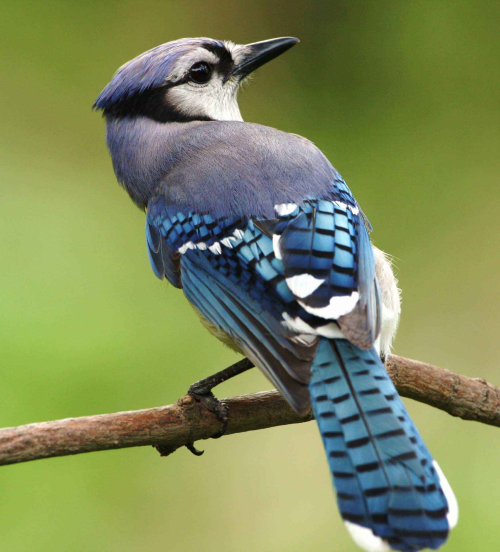
\includegraphics[width=0.5\textwidth]{bird1}
        \caption{Это типа какая-то птица}
        \label{fig:bird1}
    \end{figure}

Теперь продемонстрируем, как будут выглядеть длинные многострочные подписи. Для этого посмотрим на вторую неизвестную нам птицу, представленную на \hyperref[fig:bird2]{Рисунке \ref*{fig:bird2}}. Кстати, тут задан другой размер рисунка --- одна третья от ширины страницы.

    \begin{figure}[ht]
        \centering
        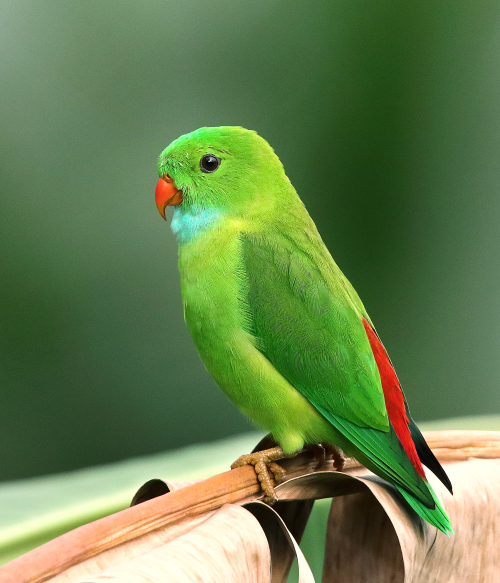
\includegraphics[width=0.33\textwidth]{bird2}
        \caption{Это другая птица, которая отличается от первой птицы формой клюва, цветом оперения, ареалом обитания, а также умением повторять за своим владельцем. Последнее, однако, не точно: птица, конечно, похожа на папугая, но мы не можем знать наверняка}
        \label{fig:bird2}
    \end{figure}

Мы напишем тут какой-нибудь текст, чтобы было видно величину отступа после подписи к рисунку. Мы не меняли это значение, оставили то, которое установлены в данном классе по умолчанию.

\subsection{Сложные многоуровневые рисунки}
\label{subsec:comp-fig}

Теперь посмотрим на то, как делать сложные рисунки. Обычно речь идет о двух-трех-четырех подрисунках, которые нумеруют (а), (б) и так далее. Мы делаем это при помощи среды \verb|subfigure| и инструментов, которые нам дает пакет \verb|subcaption|. На примере \hyperref[fig:tiger]{Рисунка \ref*{fig:tiger}} посмотрим, как задавать геометрию и расположение рисунков. Здесь два изображения разного формата, поэтому мы вручную выровняли их по высоте.

\begin{figure}[ht]
	\centering
\hspace*{\fill}%
	\begin{subfigure}[b]{0.49\textwidth}
        \centering
		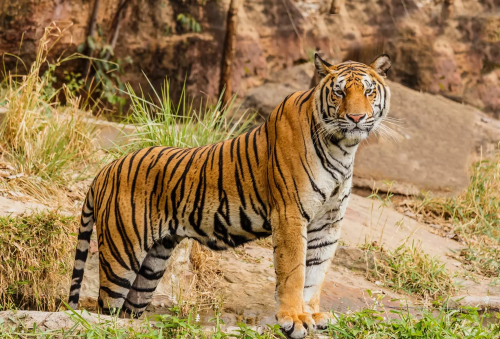
\includegraphics[height=5cm,keepaspectratio]{tiger1}
		\caption{}
		\label{fig:tiger1}
	\end{subfigure}
\hfill
	\begin{subfigure}[b]{0.49\textwidth}
        \centering
		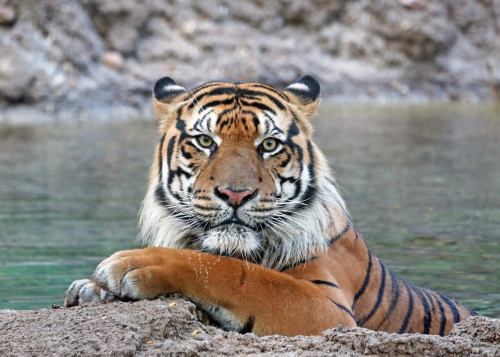
\includegraphics[height=5cm,keepaspectratio]{tiger2}
        \caption{}
		\label{fig:tiger2}
	\end{subfigure}
\hspace*{\fill}%
	\caption{Тигры. На рисунке (а) представлен гуляющий в саванне тигр, а на рисунке \\ (б) --- купающийся в водоеме. Тигр на (б) выглядит весьма довольным}
	\label{fig:tiger}
\end{figure}

Обратите внимание, что при помощи уже известных нам инструмеров можно обращаться не только в целом к рисункам, но и к конкретным подрисункам. Например, отметим, насколько же мощны лапищи этого прекрасного тигра на \hyperref[fig:tiger2]{Рисунке \ref*{fig:tiger2}}. Далее мы посмотрим, как делать двухэтажные рисунки. Добавим еще один рисунок внизу по центру. \LaTeX{} может сам менять местами рисунки и окружающий их текст с целью избежать пустых мест на страницах.

\begin{figure}[!ht]
	\centering
\hspace*{\fill}%
	\begin{subfigure}[b]{0.33\textwidth}
        \centering
		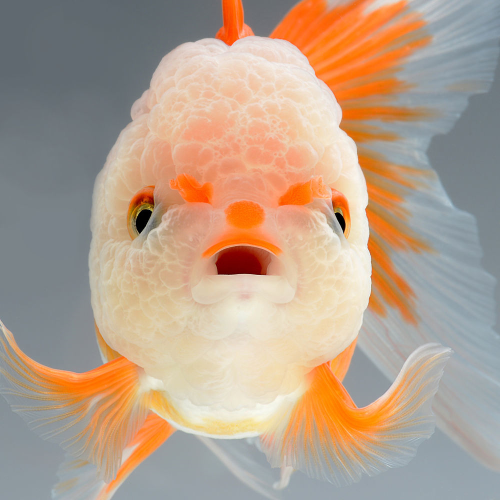
\includegraphics{fish1}
		\caption{}
		\label{fig:fish1}
	\end{subfigure}
\hfill
	\begin{subfigure}[b]{0.33\textwidth}
        \centering
		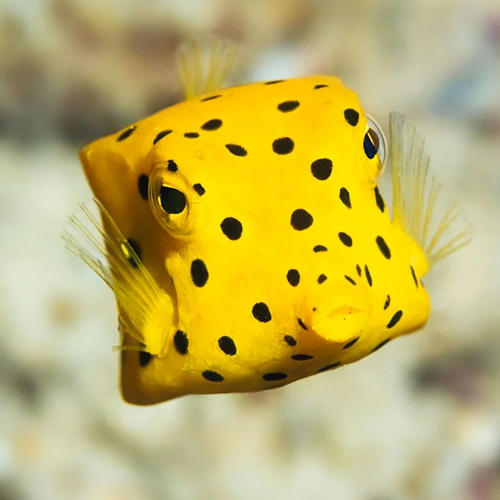
\includegraphics{fish2}
        \caption{}
		\label{fig:fish2}
	\end{subfigure}
\hspace*{\fill}%
\par\vspace{\abovecaptionskip}
        \begin{subfigure}[b]{0.33\textwidth}
        \centering
		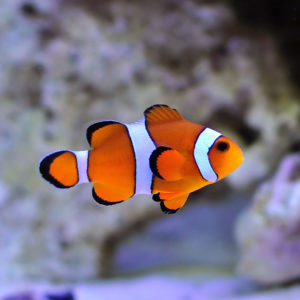
\includegraphics{fish3}
		\caption{}
		\label{fig:fish3}
	\end{subfigure}
	\caption{Разные рыбы}
	\label{fig:fish}
\end{figure}

На \hyperref[fig:fish]{Рисунке \ref*{fig:fish}} есть три фотографии одинакового размера, причем третья находится в нижнем ряду по центру. Нехитрым образом можем также сделать ссылку, которая обращается будто бы сразу к нескольким подрисункам, хотя в действительности ведет на весь рисунок. Например, можем написать так: \hyperref[fig:fish]{Рисунок \ref*{fig:fish}а--в}.

\section{Формулы}
\label{sec:equ}

Тут все просто, можете погуглить, как делать формулы, какие пакеты надо для этого подгружать, и т.д. Формулы можно вставлять прямо в текст, это делается при помощи одинарных знаков \verb|$|. Например, можно сделать вот такую штуку: $x = \frac{-b \pm \sqrt{b^2-4ac}}{2a}$. На такие формулы неудобно ссылаться. Можно сделать формулу на отдельной строке, присвоить ей номер и метку, чтобы потом обращаться к этой формуле из любого места в тексте при помощи уже известной нам команд \verb|ref| и \verb|hyperref|. Для этого есть среда \verb|equation|. Запишем выражение:
\begin{equation}
\label{eq:e1}
\frac{n!}{k!(n-k)!} = \binom{n}{k}.
\end{equation}
После этого в тексте можно ссылаться точно так же на Выражение \ref{eq:e1}, что часто оказывается весьма полезно. Можно использовать и \verb|hyperref|, сделав ссылку на \hyperref[eq:e1]{Выражение \ref*{eq:e1}} --- выбирайте сами.

Кстати, можно еще делать красивые химические реакции. В качестве примера рассмотрим \hyperref[eq:e2]{Выражение \ref*{eq:e2}}. Для создания таких выражений используется пакет \verb|mhchem|.
\begin{equation}
    \label{eq:e2}
    \ce{Na2SO4 ->[H2O] Na+ + SO4^2-}.
\end{equation}

\endinput                                     % Вторая глава
\chapter{Таблицы}
\label{ch:tab}
    Наконец, разберемся с таблицами. В принципе, \LaTeX{} позволяет делать большие и сложные таблицы, но вручную обычно их не пишут; для этого используют разные сайты типа \href{https://www.tablesgenerator.com/}{типа такого}. По ГОСТ заморачиваться с таблицами особо не надо, главное чтобы правильно были заданы подписи, работала нумерация и ссылки. Все необходимые стилевые условия уже зашиты в данный шаблон. Помните, что в конце заголовка таблицы, как и в конце подписи к рисунку, точка не ставится! Воспользовавишись сайтом по данной выше ссылке, можем сделать, например, такую таблицу:
\begin{table}[ht]
\caption{Вот так выглядит рандомная таблица из Интернета с ценой разных животных, которых можно найти в мире}
\label{tab:t1}
\centering
\begin{tabular}{llr}
\hline
Animal    & Description & Price (\$) \\ \hline
Gnat      & per gram    & 13.65      \\
          & each        & 0.01       \\
Gnu       & stuffed     & 92.50      \\
Emu       & stuffed     & 33.33      \\
Armadillo & frozen      & 8.99       \\ \hline
\end{tabular}
\end{table}

На эту таблицу, безусловно, можно так же ссылаться. Давайте сошлемся на \hyperref[tab:t1]{Таблицу \ref*{tab:t1}} и на этом, пожалуй, закончим.

\endinput                                     % Третья глава

\printbibliography[title=Список использованных источников] % Автособираемый список литературы

\end{document}